%
% einleitung.tex -- Beispiel-File für die Einleitung
%
% (c) 2020 Prof Dr Andreas Müller, Hochschule Rapperswil
%
% !TEX root = ../../buch.tex
% !TEX encoding = UTF-8
%
\section{Mathematisches Grundgerüst\label{mongekant:section:teil0}}
\kopfrechts{Mathematisches Grundgerüst}

Um die Modelle des optimalen Transports zu verstehen,
müssen wir uns zunächst mit einigen mathematischen Grundlagen vertraut machen.
Damit die Konzepte klar werden,
werden wir die Theorie anhand eines anschaulichen Beispiels mit Sandhaufen erläutern.
\index{Sandhaufen}%

\subsection{Transport von Masse\label{mongekant:subection:transport}}
Stellen wir uns vor,
wir wollen einen Sandhaufen vom Raum $X$
in den Raum $Y$ transportieren.
Dabei möchten wir vielleicht auch gerade die Form des Haufens ändern.
Eine Teilmenge $A\subset X$ des Quellhaufens enthält die Masse $\mu(A)$,
was man sich als die Masse einer Schaufel Sand vorstellen kann.
Analog enthält eine Teilmenge $B\subset Y$ des Zielhaufens die Masse $\nu(B)$.

Der Transport wird durch eine Abbildung
\begin{align*}
T\colon X\to Y
,\qquad y=T(x)
\end{align*}
beschrieben,
die jedem Punkt $x\in X$ einen Zielpunkt $y\in Y$ zuordnet.
Damit die Masse beim Transport erhalten bleibt,
muss für jede messbare Teilmenge $B\subset Y$
\begin{align*}
\nu(B)
&=
\mu(A)
\\
&=
\mu\left(T^{-1}(B)\right)
=
T_{\#}\mu(B)
\end{align*}
gelten.
$T_{\#}\mu$ wird in der Literatur als \emph{Push-Forward} von $\mu$ nach $\nu$ durch $T$ bezeichnet.
\index{Push-Forward}%
In Abbildung~\ref{mongekant:fig:optimal_transport} ist der 1-dimensionale Fall dargestellt.

\begin{figure}
\centering
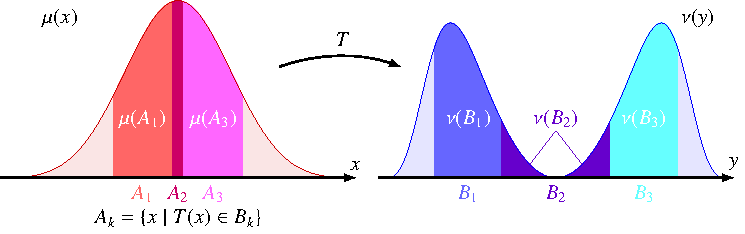
\includegraphics{papers/mongekant/images/t}
\caption{1-dimensionaler Transport von $\mu(A_k)$ nach $\nu(B_k)$ mittels Abbildung $T$}
\label{mongekant:fig:optimal_transport}
\end{figure}

In vielen Anwendungen sind $\mu$ und $\nu$ Wahrscheinlichkeitsmasse,
also gilt
\begin{align*}
\mu(X)
&=
\nu(Y)
=
1
.
\end{align*}
%Befindet sich $\mu$ (bzw. $\nu$) im
Im sogenannt absolut stetigen Fall
existieren Dichten $f,g\in L^{1}$ mit
\begin{align}
\begin{aligned}
\mu(A)
&=
\int_A f(x) \, dx
\\
\nu(B)
&=
\int_B g(y) \, dy
.
\end{aligned}
\label{mongekant:eq:absolute_continuity}
\end{align}
Ist $T$ differenzierbar, liefert die Variablensubstitutionsformel im Integral
die Bedingung
\[
\int_B g(y)\,dy
=
\int_{T^{-1}(B)} g(T(x))\, T'(x)\,dx
=
\int_A f(x)\,dx
\qquad\Rightarrow\qquad
g(T(x))\, T'(x) = f(x)
\]
in Form einer nichtlinearen Differentialgleichung für die Funktion $T$.

\subsection{Kosten des Transports\label{mongekant:subsection:transport_cost}}
Nun stellt sich die Frage,
wie ``teuer'' der Transport von $A$ nach $B$ ist.
Dazu führen wir eine Kostenfunktion $c : X \times Y \to [0, +\infty]$ ein,
\index{Kostenfunktion}%
die die Kosten $c(x,y)$ für den Transport eines Sandkorns
von $x \in X$ nach $y \in Y$ angibt.
\index{Sandkorn}%
Die Gesamtkosten $C$ für den Transport $T$ von $X$ nach $Y$ sind dann
\index{Gesamtkosten}%
\begin{align}
C(T)
&=
\int_X c\bigl(x, T(x)\bigr) \, d\mu(x)
\label{mongekant:eq:monge_transport_cost}
.
\end{align}
Die Schreibweise $d\mu(x)$ ist die übliche Formulierung des
Lebesgue-Integrals über ein beliebiges Mass.
\index{Lebesgue-Integral}%
Man kann sich $d\mu(x)$ als ``infinitesimale Masse'' vorstellen,
die an der Stelle $x$ liegt.
Oder um unsere Sandhaufen-Analogie zu verwenden,
die Masse eines einzelnen Sandkorns.
In der Literatur wird manchmal die alternative Schreibweise $\mu(dx)$ verwendet,
diese suggeriert jedoch fälschlicherweise, dass die Masse unabhängig vom Ort ist,
was im Allgemeinen nicht der Fall ist.
Deshalb benutzen wir ausschliesslich die Schreibweise $d\mu(x)$.
